\chapter{Technologia CUDA}

CUDA (Compute Unified Device Architecture) to architektura stworzona przez firmę NVIDIA. Pozwala ona na programowanie odpowiednich kart graficznych w sposób umożliwiający wykonywanie obliczeń ogólnego przeznaczenia. Programy napisane z wykorzystaniem technologii CUDA zasadniczo różnią się od standardowych programów, które są wykonywane na zwykłych procesorach. Swoją charakterystyką przypominają one bardziej programy równoległe, które są wykonywane na klastrach obliczeniowych, niż standardowe programy sekwencyjne. CUDA pozwala na wykorzystanie architektury karty graficznej (Rysunek~\ref{fig:GPU Devotes More Transistors to Data Processing}) w celu wykonania obliczeń w sposób zauważalnie odmienny niż w przypadku procesora.
\begin{figure}
    \centering
    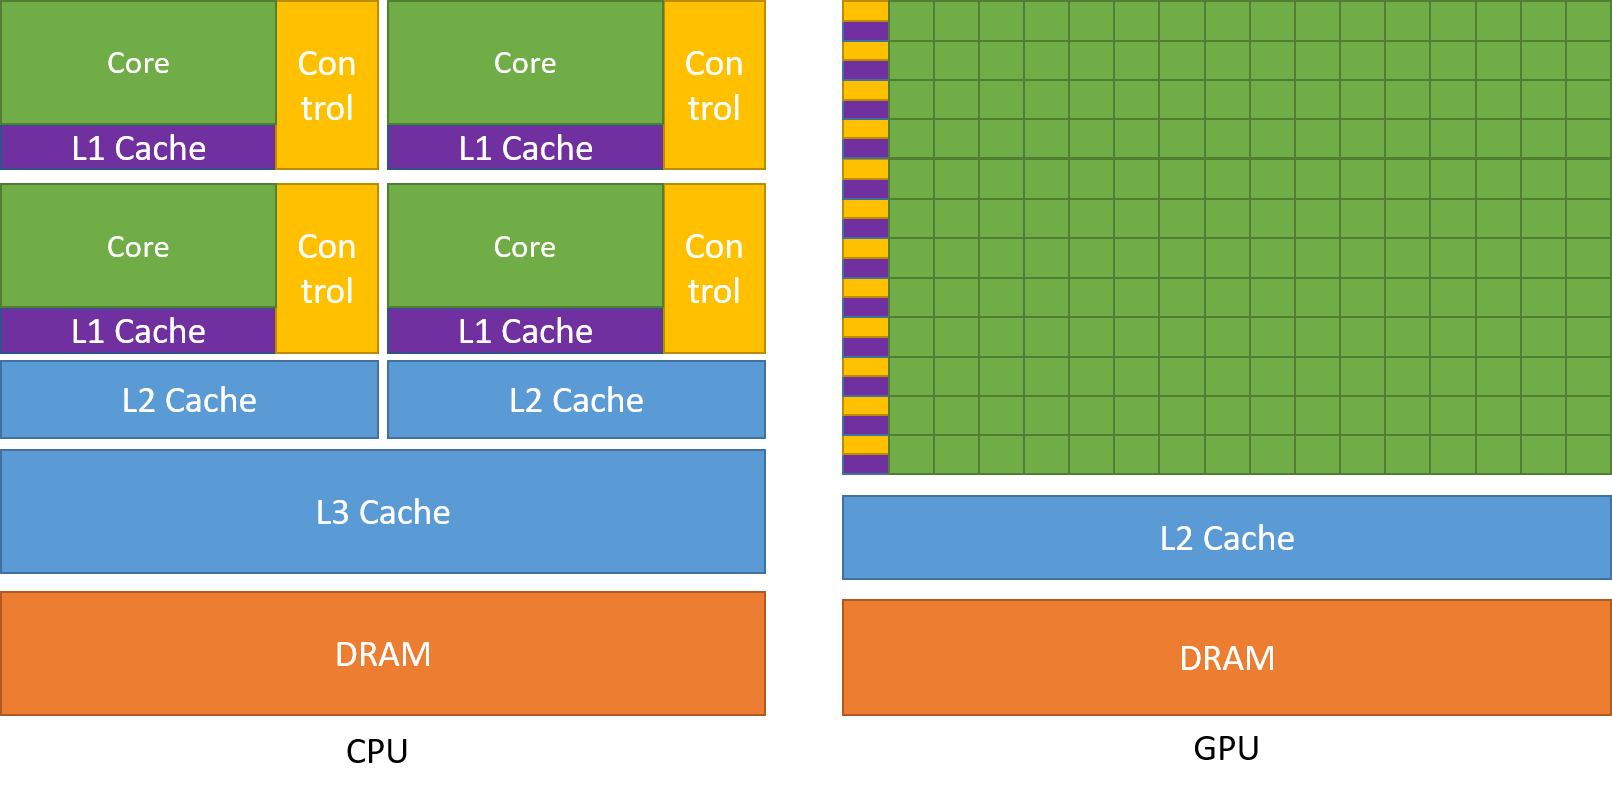
\includegraphics[scale=0.5]{./fig/gpu-devotes-more-transistors-to-data-processing.png}
    \caption{docs.nvidia.com - "GPU Devotes More Transistors to Data Processing", ilustracja różnicy w architekturze procesora i karty graficznej}
    \label{fig:GPU Devotes More Transistors to Data Processing}
\end{figure}

\section{Model programowania}
W przeciwieństwie do programowania wielowatkowego na CPU, programowanie w technologii CUDA nie polega na zarządzaniu każdym wątkiem oddzielnie, a całym blokiem wątków naraz. Wątki w bloku są grupowane w tzw. \textit{warp}, czyli grupę 32 wątków, które są wykonywane równolegle. Bloki wątków są grupowane w \textit{grid} - siatkę bloków, która jest wykonywana na karcie graficznej. Model programowania w technologii CUDA jest zilustrowany na Rysunku~\ref{fig:Grid of Thread Blocks}. Pozwala to wykonywać jednocześnie tę samą operację na wielu elementach danych przy wykorzystaniu rdzeni CUDA. W ten sposób możliwe jest uzyskanie znacznie większej wydajności obliczeń niż w przypadku wykonywania ich sekwencyjnie na procesorze. Architektura GPU narzuca jednak pewne ograniczenia. Możliwość wykonania obliczeń na tysiącach wątków jednocześnie, osiągnięto kosztem możliwości pojedynczego wątku. Wątki na GPU nie mogą komunikować się bezpośrednio między sobą, co w połączeniu z ich ilością, wynosi problem konkurencyjności obliczeń na wyższy poziom abstrakcji niż w przypadku programowania wielowątkowego na CPU. Architektura sprawia również, że operacje warunkowe w kodzie CUDA mogą znacząco obniżyć wydajność urządzenia. W przypadku rozgałęzienia w kodzie CUDA, jeżeli jeden wątek spełni warunek rozgałęzienia, wtedy wszystkie wątki wchodzące w dany warp będą musiały czekać na zakończenie obliczeń przez ten pojedynczy wątek. W pesymistycznym przypadku może to oznaczać, że w danym momencie dysponujemy jedyni 1/32 mocy obliczeniowej karty graficznej.
\begin{figure}
    \centering
    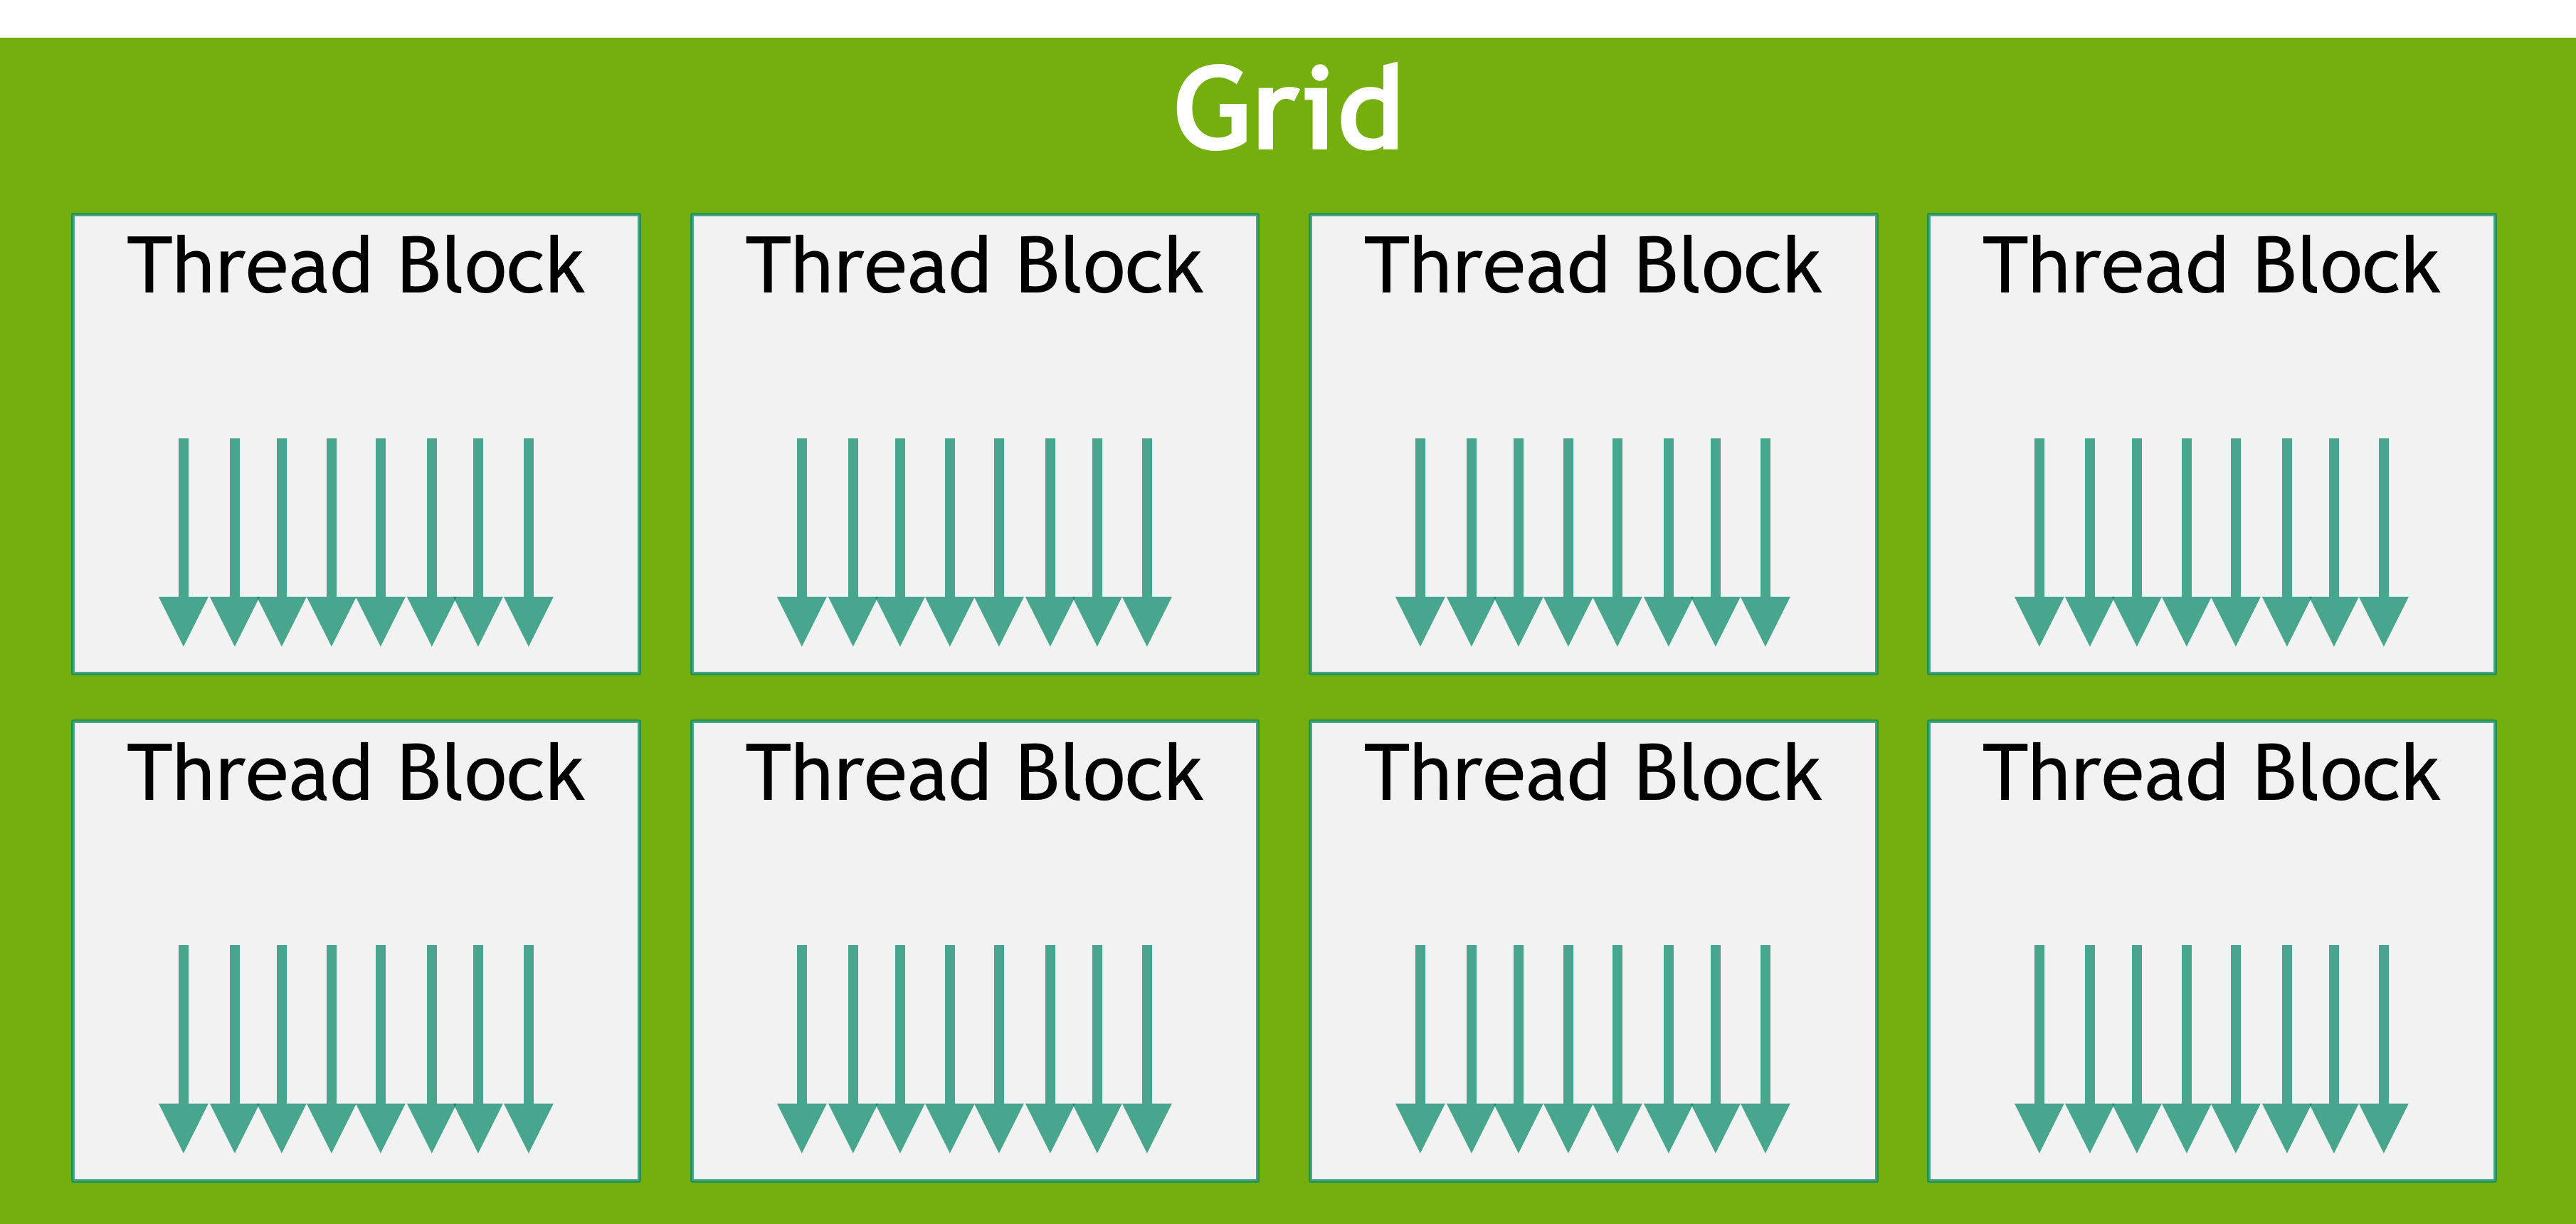
\includegraphics[scale=0.5]{./fig/grid-of-thread-blocks.png}
    \caption{docs.nvidia.com - "Grid of Thread Blocks", ilustracja modelu programowania w technologii CUDA}
    \label{fig:Grid of Thread Blocks}
\end{figure}

\begin{figure}
    \centering
    % 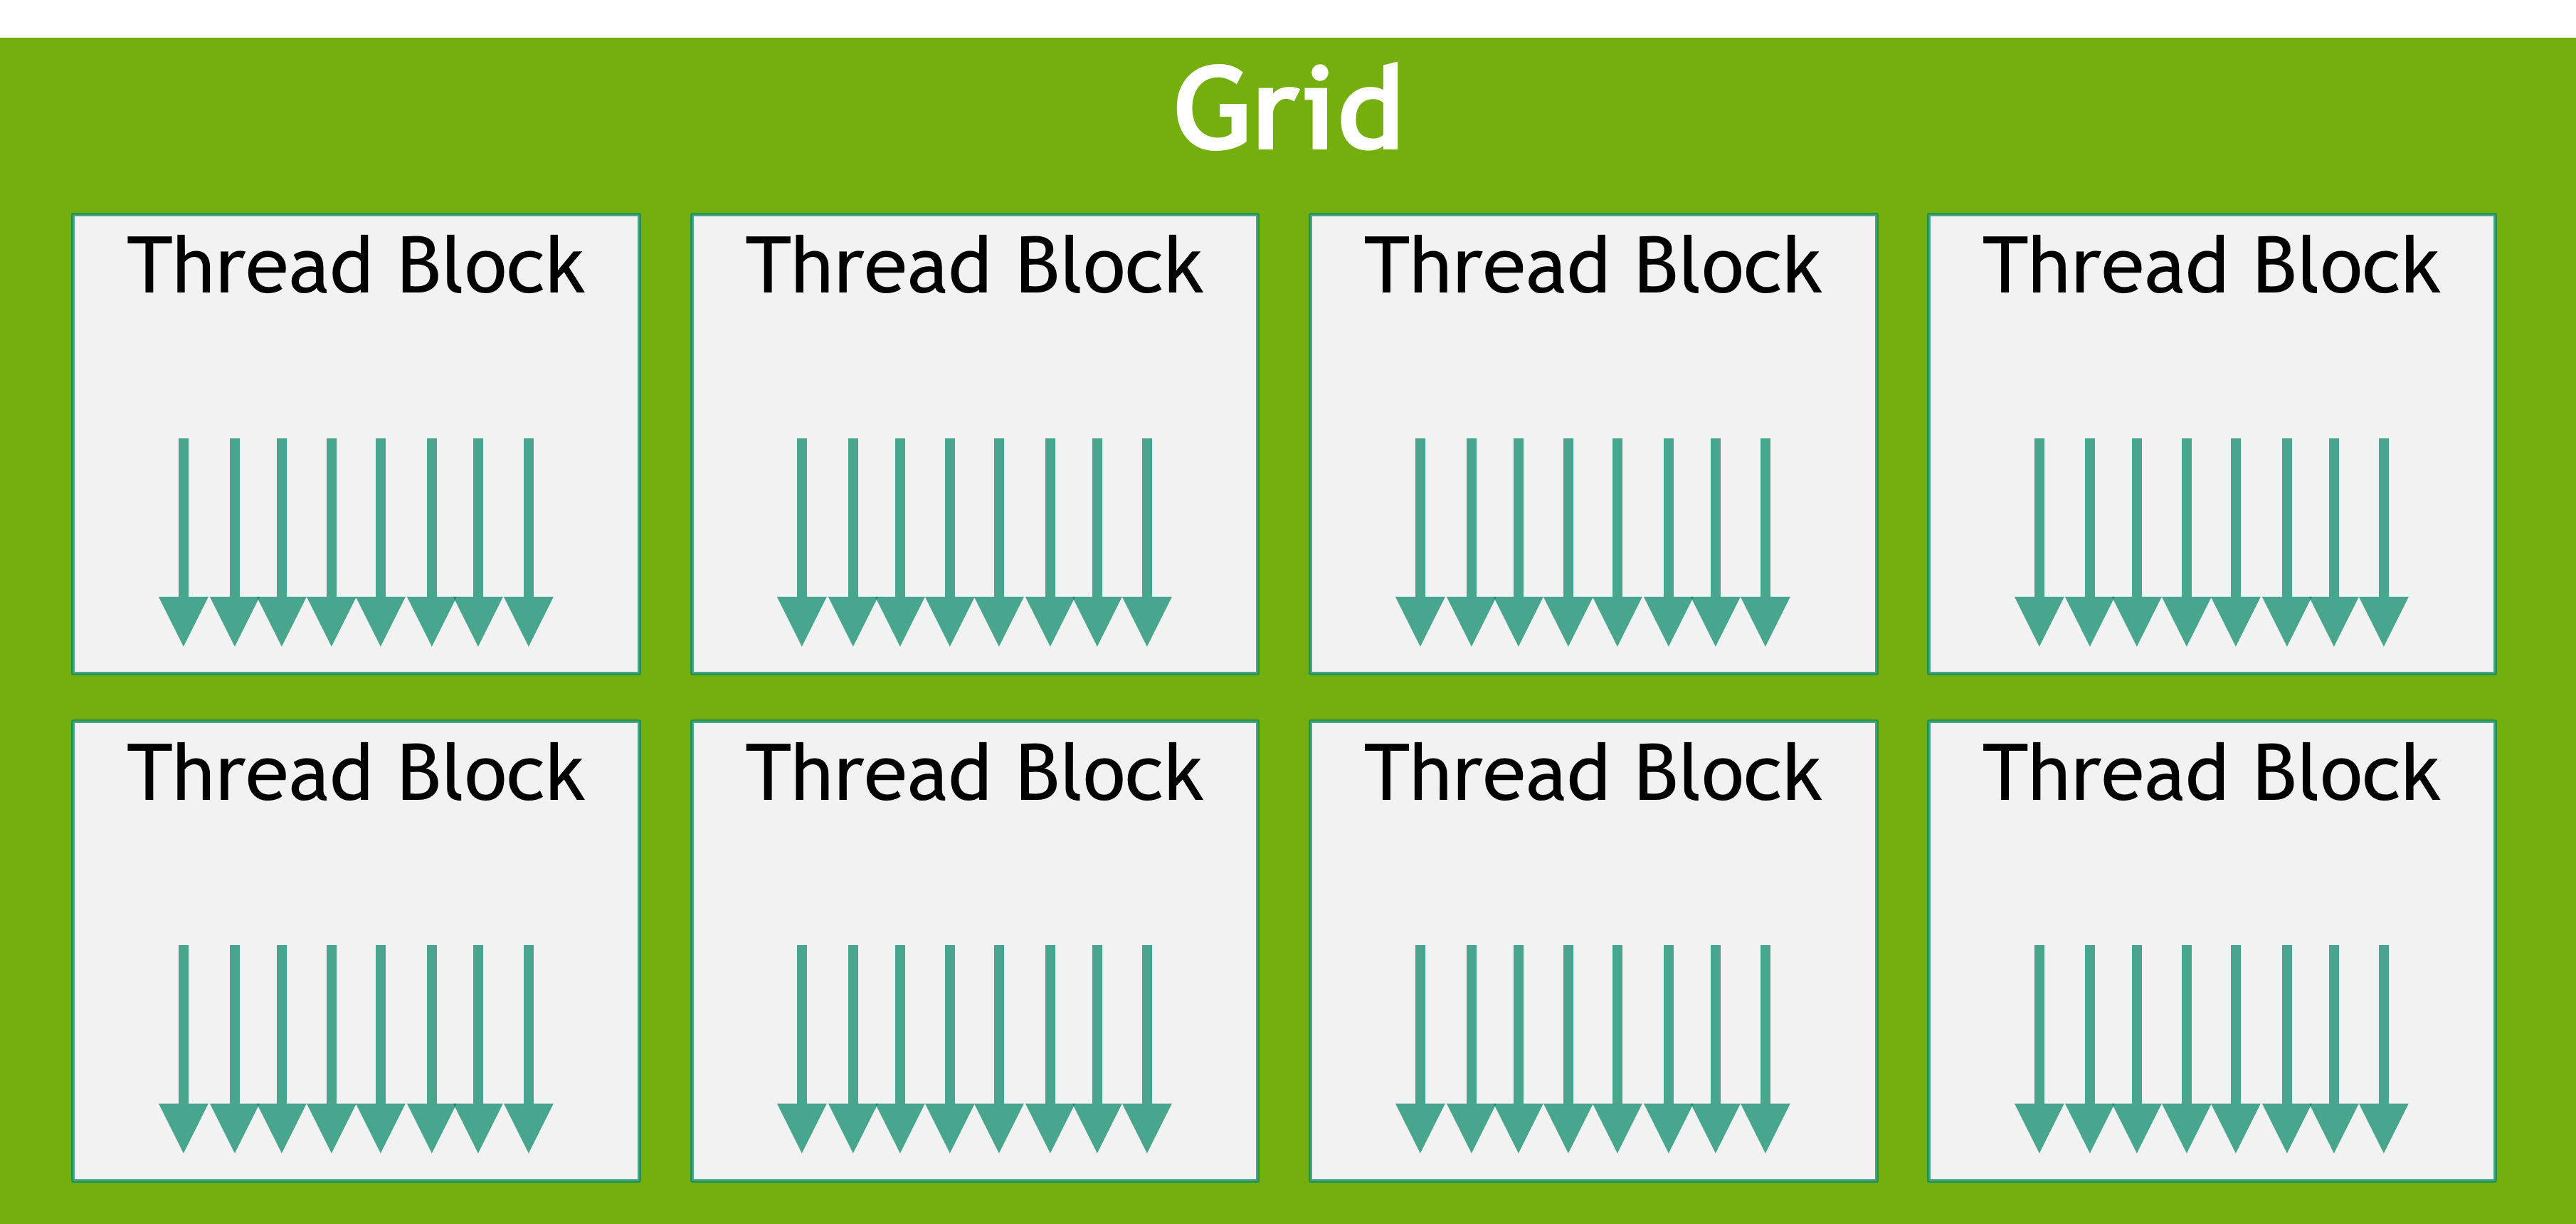
\includegraphics[scale=0.5]{./fig/grid-of-thread-blocks.png}
    \caption{Przykładowe wywołanie kernela CUDA}
    \label{fig:Przykładowe wywołanie kernela CUDA}
\end{figure}

\section{Host i Device}
Urządzenie GPU można traktować jako oddzielny komputer, posiadający swoje własne podzespoły oraz zasoby. Technologia CUDA właśnie w ten sposób reprezentuje kompatybilną kartę graficzną. Interfejs programistyczny CUDA rozróżnia dwa środowiska: \textit{host} oraz \textit{device}. Host to komputer, na którym uruchamiany jest program, który wykorzystuje technologię CUDA. Device to karta graficzna, na której wykonywane są obliczenia. Najbardziej podstawowym schematem programu wykorzystującego tą technologię jest: przekazanie danych przygotowanych na urządzeniu host do urządzenia device, które wykonuje obliczenia. Po zakończeniu obliczeń, urządzenie host pobiera wyniki z GPU, gdzie możliwa jest ich interpretacja, zapis lub dalsze przetwarzanie. Można zauważyć, iż na moc obliczeniową, wynikającą z połączenia CPU oraz GPU, składa się również szybkość przesyłania danych między tymi dwoma urządzeniami. Tabela \ref{tab:Przepustowość przsyłu danych} przedstawia przeciętne możliwości w kategorii kopiowania danych zawartych w konkretnych typach pamięci urządzeń. Należy zauważyć ograniczenia jakie za sobą niesie wykorzystywanie szyny PCIE w przypadku intensywnej komunikacji pomiędzy CPU a GPU. Sugerowanym przez NVIDIA'e rozwiązaniem jest przekazanie jedynie niezbędnych danych w celu wykonania obliczeń na GPU, a następnie zwrócenie jedynie samego wyniku obliczeń. W ten sposób można przynajmniej częściowo zniwelować efekt wąskiego gardła, jaki może wynikać z przepustowości szyny PCIE. Alternatywnym rozwiązaniem jest wykonywanie obliczeń asynchronicznie względem przesyłu danych, co pozwala na wykonanie obu operacji w tym samym czasie i zlikwidowanie czasu oczekiwania na zakończenie przesyłu danych.


\begin{table}[t]
    \begin{center}
        \caption{Przeciętna przepustowość przesyłu danych dla danego standardu / urządzenia}
        \label{tab:Przepustowość przsyłu danych}
        \begin{tabular}{r|l|c}
            urządzenie & typ & przepustowość \\
            \hline
                       & L1 cache    & 500GB/s - 1TB/s  \\
            CPU        & L2 cache    & 200GB/s - 1TB/s  \\
                       & L3 cache    & 75GB/s - 400GB/s \\
            \hline
                       & DDR3        & 10GB/s - 20GB/s  \\
            RAM        & DDR4        & 17GB/s - 25GB/s  \\
                       & DDR5        & 35GB/s - 50GB/s  \\
            \hline
                       & L1 cache    & 1TB/s - 2TB/s    \\
            GPU        & L2 cache    & 500GB/s - 1TB/s  \\
                       & DRAM        & 200GB/s - 800GB/s\\
            \hline
                       & 3.0         & 1GB/s - 16GB/s   \\
            PCIE       & 4.0         & 2GB/s - 32GB/s   \\
                       & 5.0         & 4GB/s - 64GB/s   \\
        \end{tabular}
    \end{center}
\end{table}

% intel.com/content/www/us/en/developer/articles/technical/memory-performance-in-a-nutshell.html
% cpu-world.com/
% transcend-info.com/Support/FAQ-292

% web.archive.org/web/20140518224913/http://www.pcisig.com/news_room/faqs/FAQ_PCI_Express_4.0/#EQ3
% web.archive.org/web/20140201172536/http://www.pcisig.com/news_room/faqs/pcie3.0_faq/#EQ2

\section{Zastosowanie dla problematyki przetwarzania sygnałów}
Technologia CUDA jest obecnie wykorzystywana do przetwarzania sygnałów cyfrowych. Przy użyciu biblioteki cuFFT możliwe jest wykorzystanie mocy obliczeniowej karty graficznej do przetwarzania sygnałów w dziedzinie częstotliwości. Technologia ta nie jest jednak popularna w przypadku przetwarzania sygnałów dźwiękowych w przypadku w przemyśle rozrywkowym. Nie licząc pojedynczych prób w latach 2000 - 2010, które z powodu małej kompatybilności oprogramowania, zakończyły się niepowodzeniem, nie ma obecnie dostępnych narzędzi, wykorzystujących moc obliczeniową karty graficznej w przemyśle muzycznym. Technologia CUDA oraz karty firmy NVIDIA stały się dużo bardziej rozwinięte i popularne. W związku z tym ponowne podejście do tematu przetwarzania sygnałów dźwiękowych przy użyciu CUDA może przynieść pozytywne rezultaty. Natura popularnego w przemyśle muzycznym formatu PCM sprawia, że przetwarzanie sygnałów dźwiękowych jest zadaniem, które można wykonać przy użyciu algorytmów korzystających z równoległości. Najprostszym przykładem jest zastosowanie wykorzystanie n wątków GPU do przetworzenia n próbek sygnału zawartych w buforze. Sytuacja przedstawiona na Rysunku~\ref{fig:Wykorzystanie n wątków do przetworzenia n próbek} ilustruje metodę, którą można by bez problemu wykorzystać przy zrównoleglaniu nieskomplikowanych algorytmów. W przypadku algorytmów bardziej złożonych lub wymagających sekwencyjnego przetwarzania danych dla kolejnych próbek, może się stać niemożliwym wykorzystanie tego podejścia. Rozwiązaniem tego problemu może być zastosowanie m wątków do przetworzenia m buforów w sposób liniowy, zakładając, iż dany algorytm zostaje wywołany jednocześnie m-krotnie. Przykład takiego podejścia przedstawiono na Rysunku~\ref{fig:Wykorzystanie m wątków do przetworzenia m buforów}. O ile te rozwiązanie nie jest tak samo wydajne, co pierwsze z przedstawionych, nie koniecznie musi implementować cały algorytm, a jedynie jego problematyczną część. Idealną sytuacją byłoby wywołanie algorytmu niesekwencyjnego m-krotnie. Taki przypadek pozwalałby na wykorzystanie pełni mocy obliczeniowej karty graficznej. Przykład takiego podejścia przedstawiono na Rysunku~\ref{fig:Wykorzystanie m*n wątków do przetworzenia m buforów po n próbek}. Dobór podejścia może okazać się kluczowy dla uzyskania zadowalających wyników. Niewykluczone, iż w wielu przypadkach konieczne będzie zastosowanie hybrydowego podejścia, łączącego przedstawione metody.

\begin{figure}
    \centering
    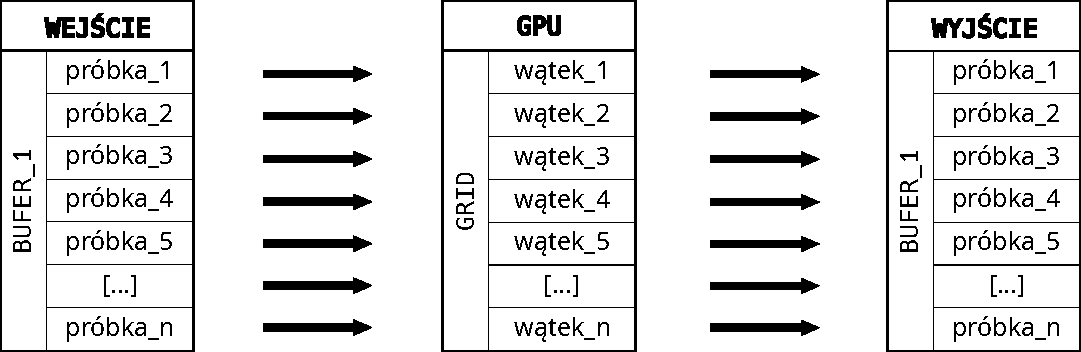
\includegraphics[width=\textwidth]{./fig/przetwarzanie_1_do_1.pdf}
    \caption{Wykorzystanie n wątków do przetworzenia n próbek}
    \label{fig:Wykorzystanie n wątków do przetworzenia n próbek}
\end{figure}

\begin{figure}
    \centering
    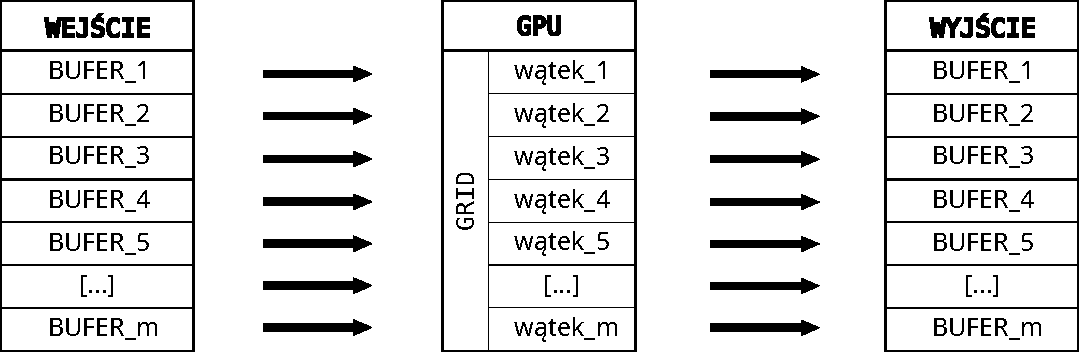
\includegraphics[width=\textwidth]{./fig/przetwarzanie_m_do_1.pdf}
    \caption{Wykorzystanie m wątków do przetworzenia m buforów w sposób liniowy}
    \label{fig:Wykorzystanie m wątków do przetworzenia m buforów}
\end{figure}

\begin{figure}
    \centering
    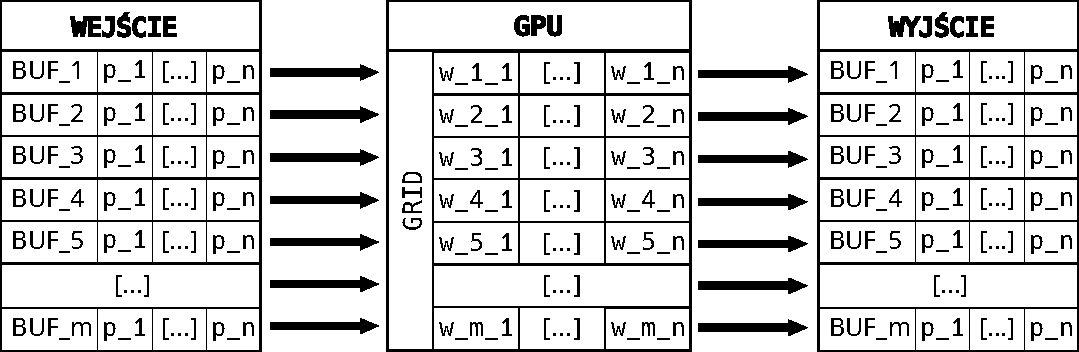
\includegraphics[width=\textwidth]{./fig/przetwarzanie_m_do_m.pdf}
    \caption{Wykorzystanie m*n wątków do przetworzenia m buforów po n próbek}
    \label{fig:Wykorzystanie m*n wątków do przetworzenia m buforów po n próbek}
\end{figure}